\begin{figure}[H]
\centering
\subfigure{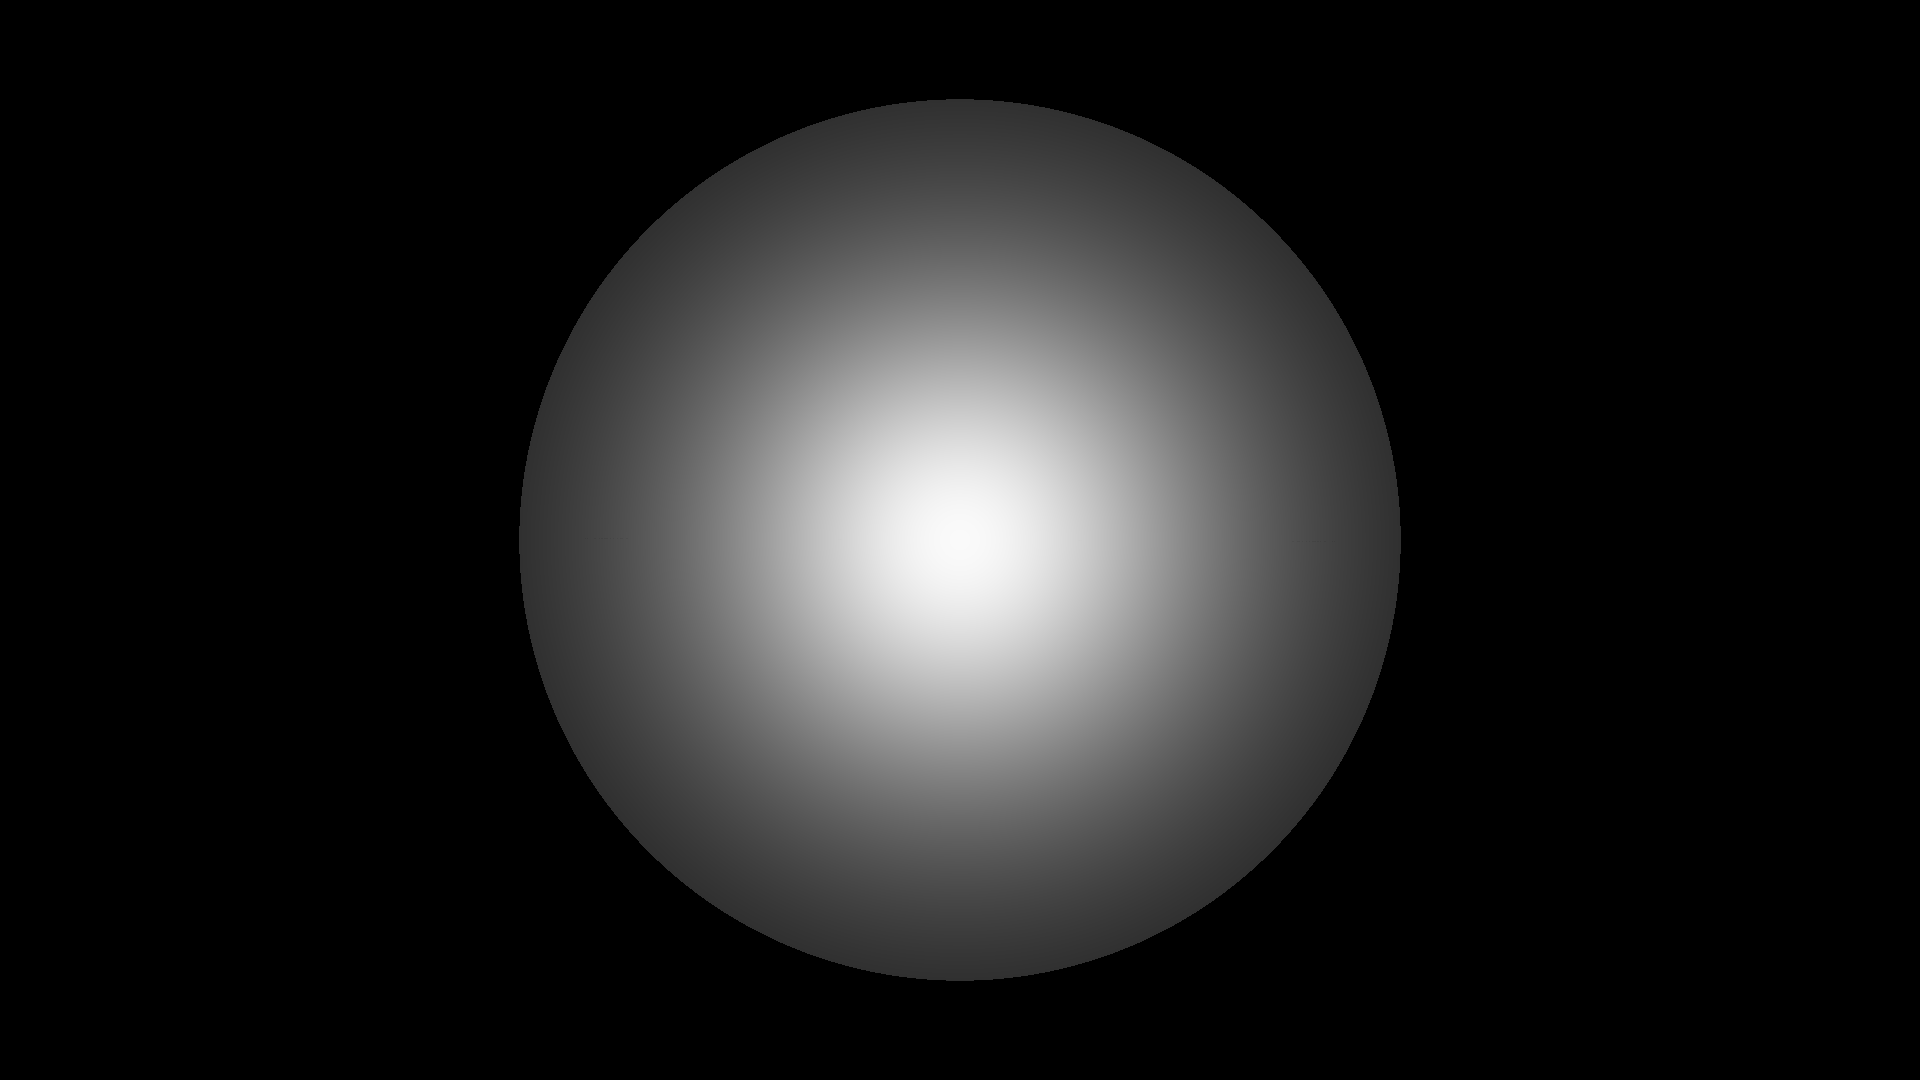
\includegraphics[width=0.3\textwidth]{chapters/ch3/img/light/output_07_07_0_0_1.png}}
\subfigure{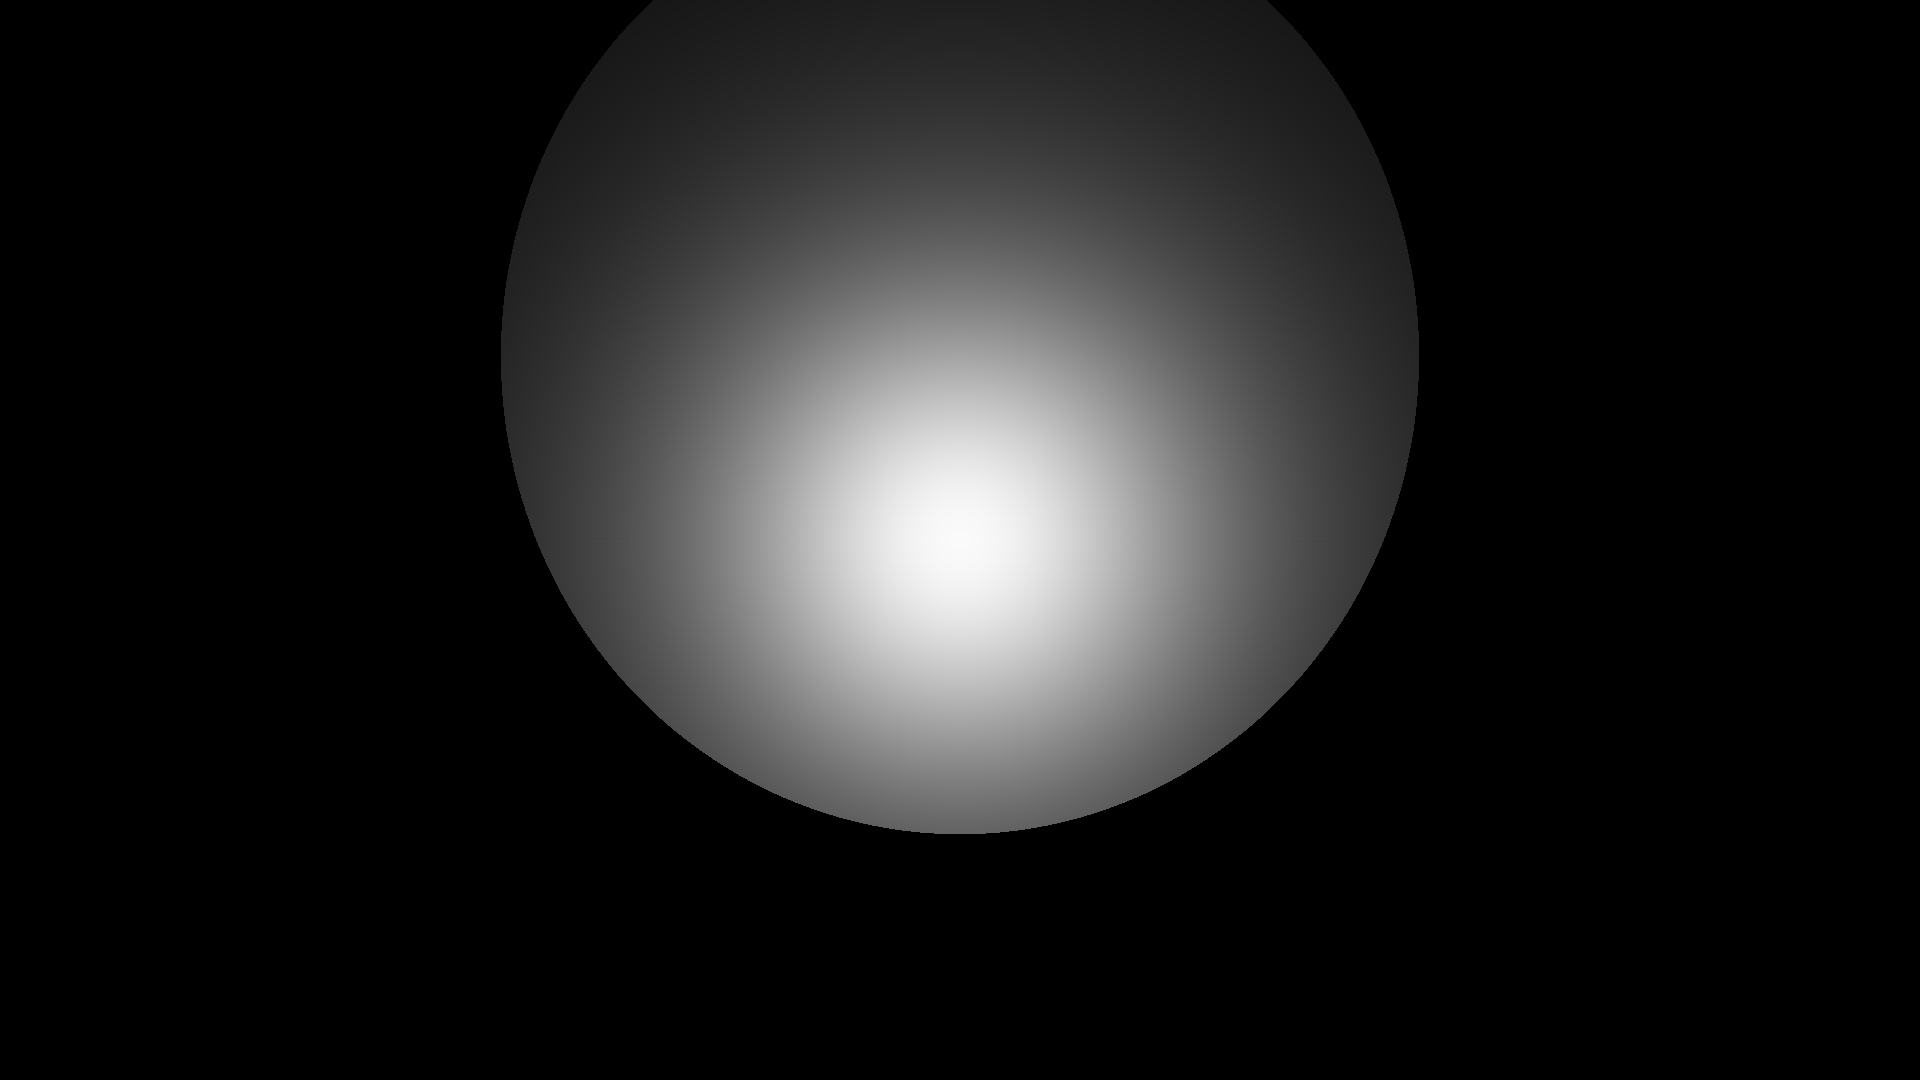
\includegraphics[width=0.3\textwidth]{chapters/ch3/img/light/output_07_07_0_02_1.png}}
\subfigure{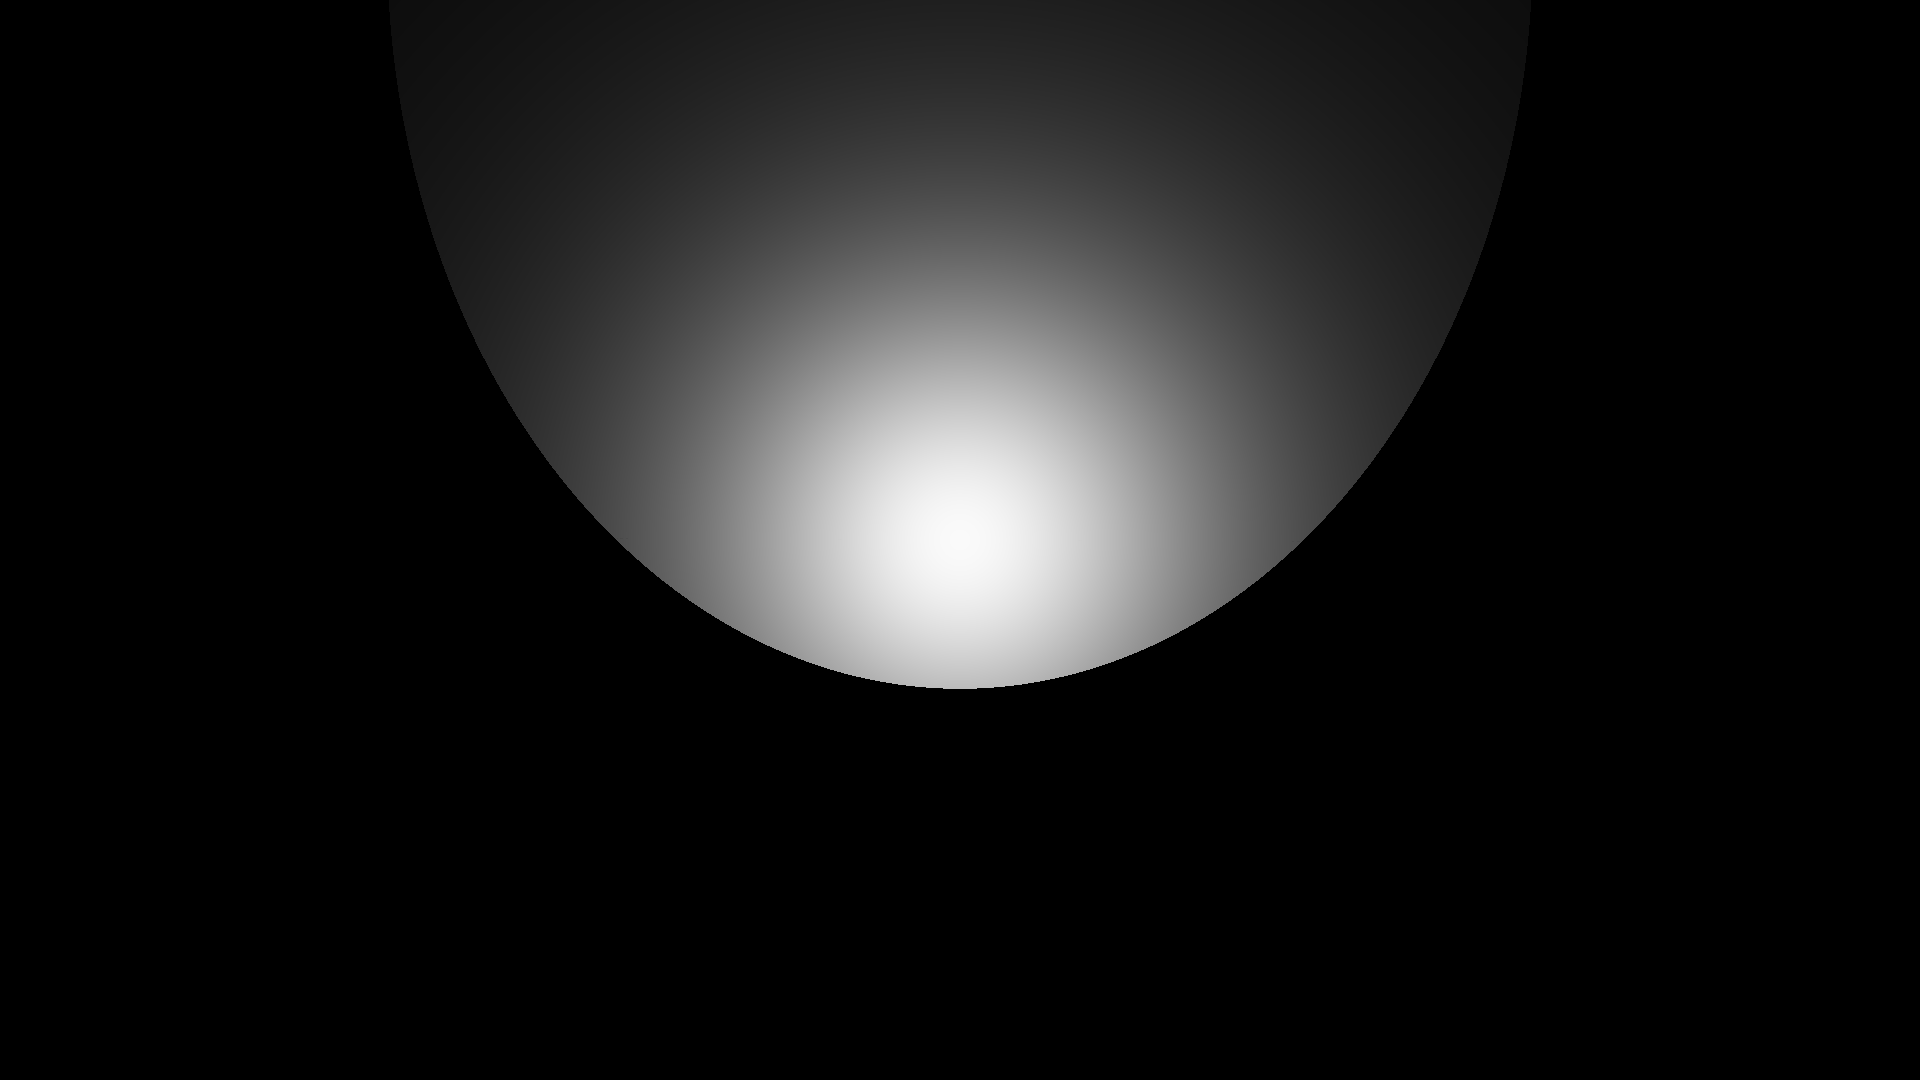
\includegraphics[width=0.3\textwidth]{chapters/ch3/img/light/output_07_07_0_05_1.png}}

\subfigure{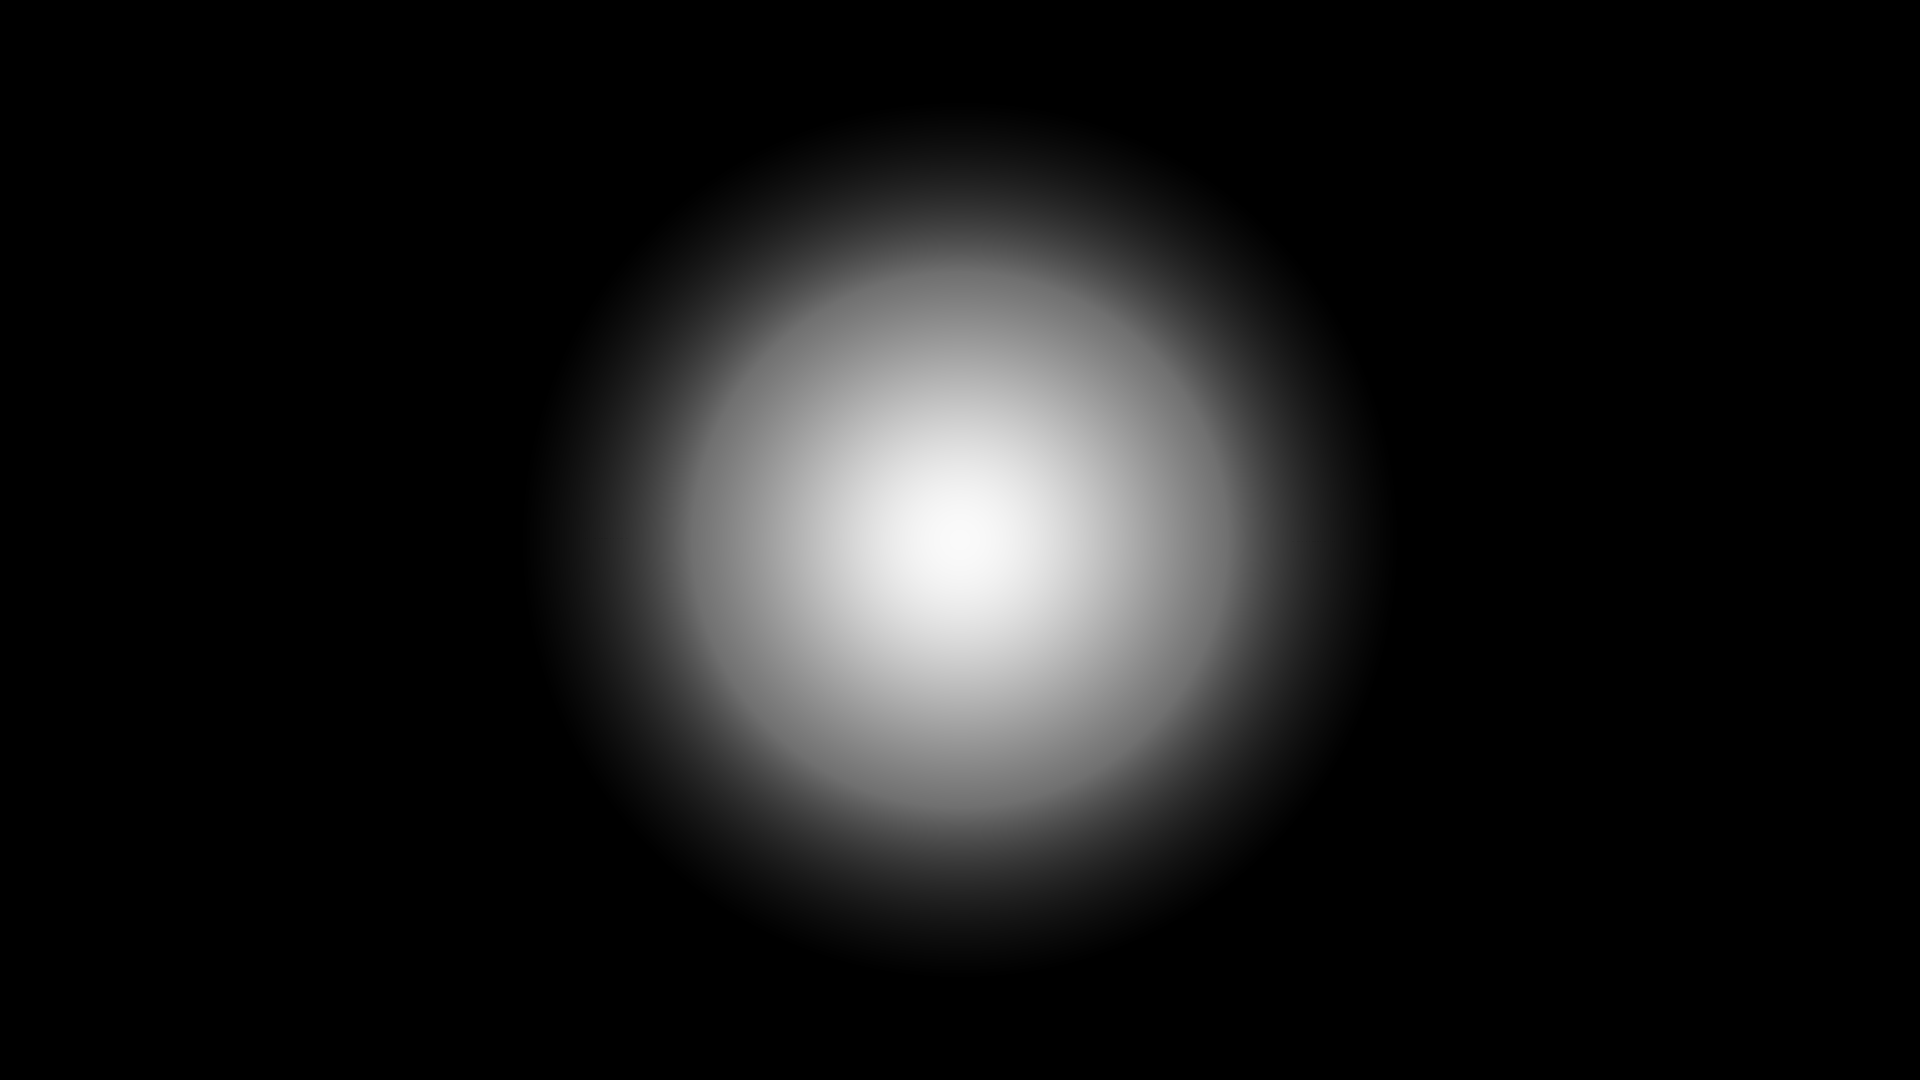
\includegraphics[width=0.3\textwidth]{chapters/ch3/img/light/output_07_085_0_0_1.png}}
\subfigure{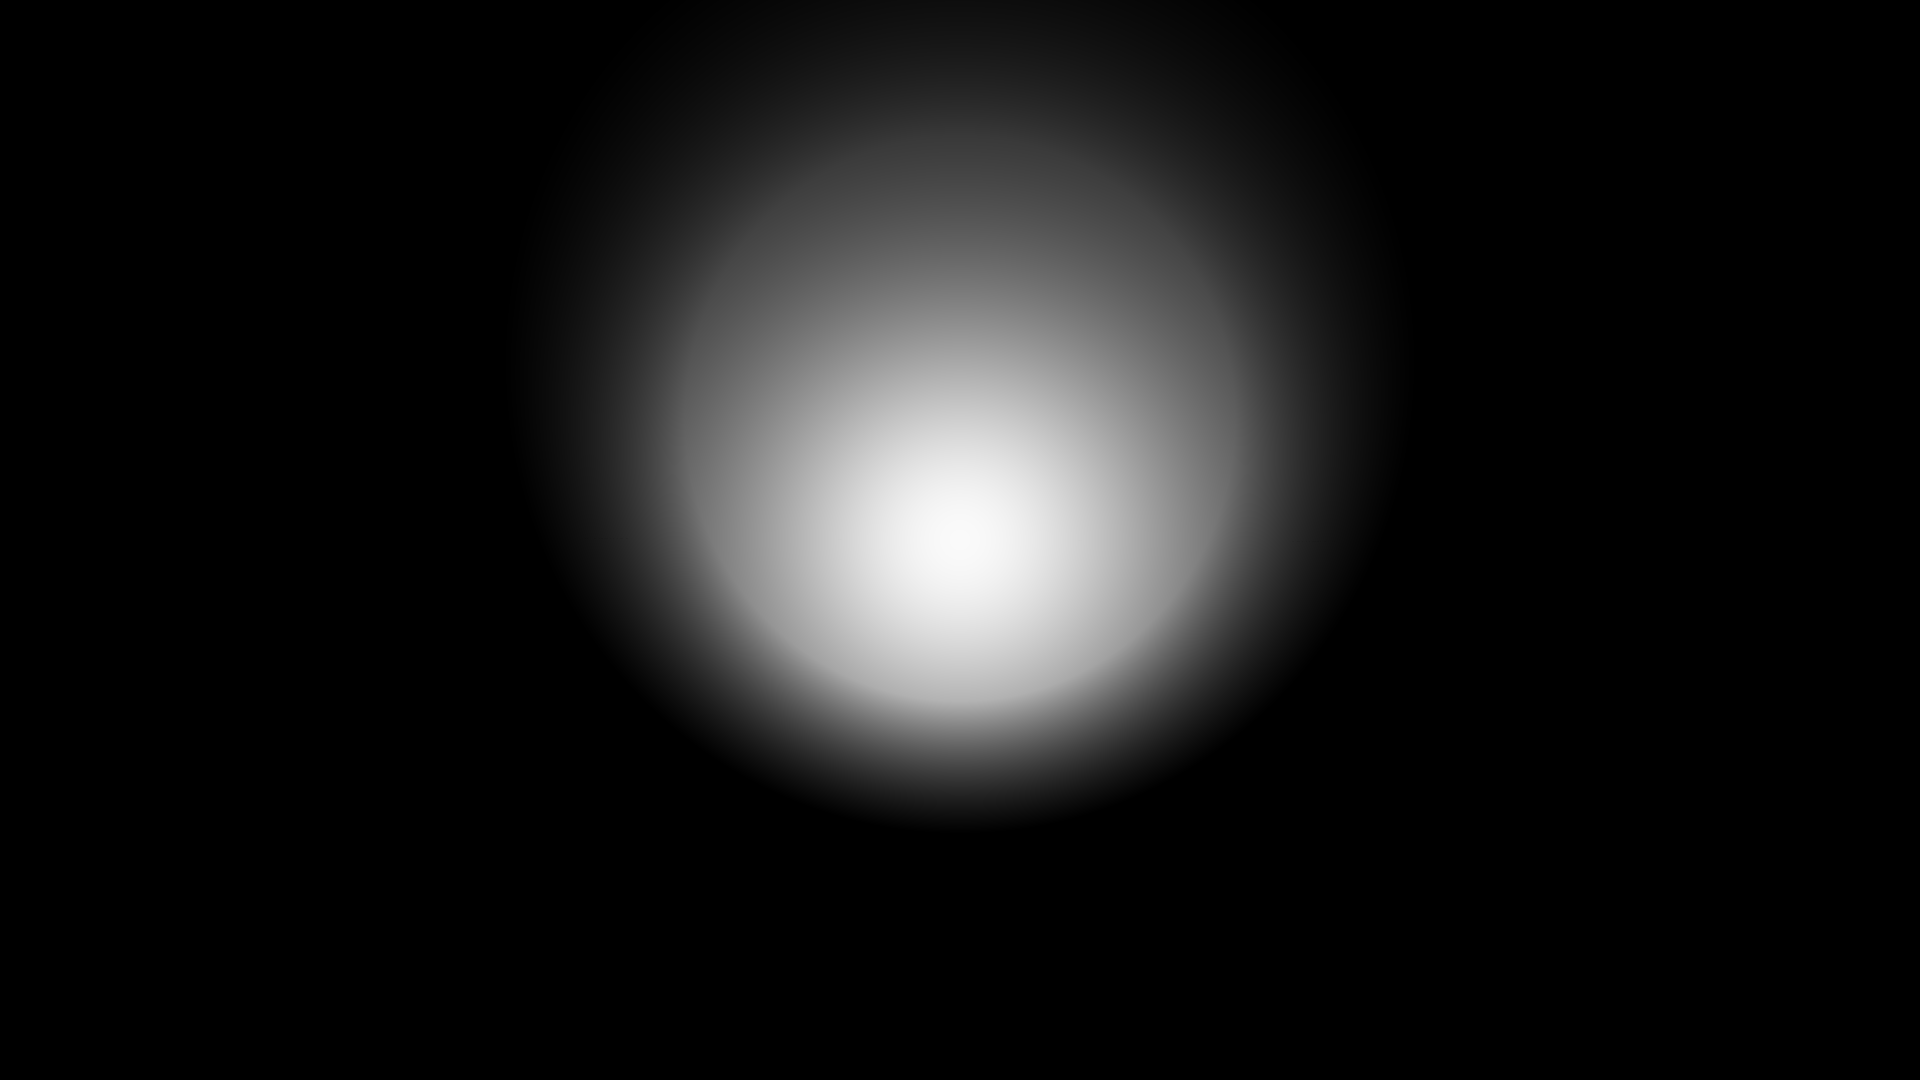
\includegraphics[width=0.3\textwidth]{chapters/ch3/img/light/output_07_085_0_02_1.png}}
\subfigure{
\includegraphics[width=0.3\textwidth]{chapters/ch3/img/light/output_07_085_0_05_1.png}}

\subfigure{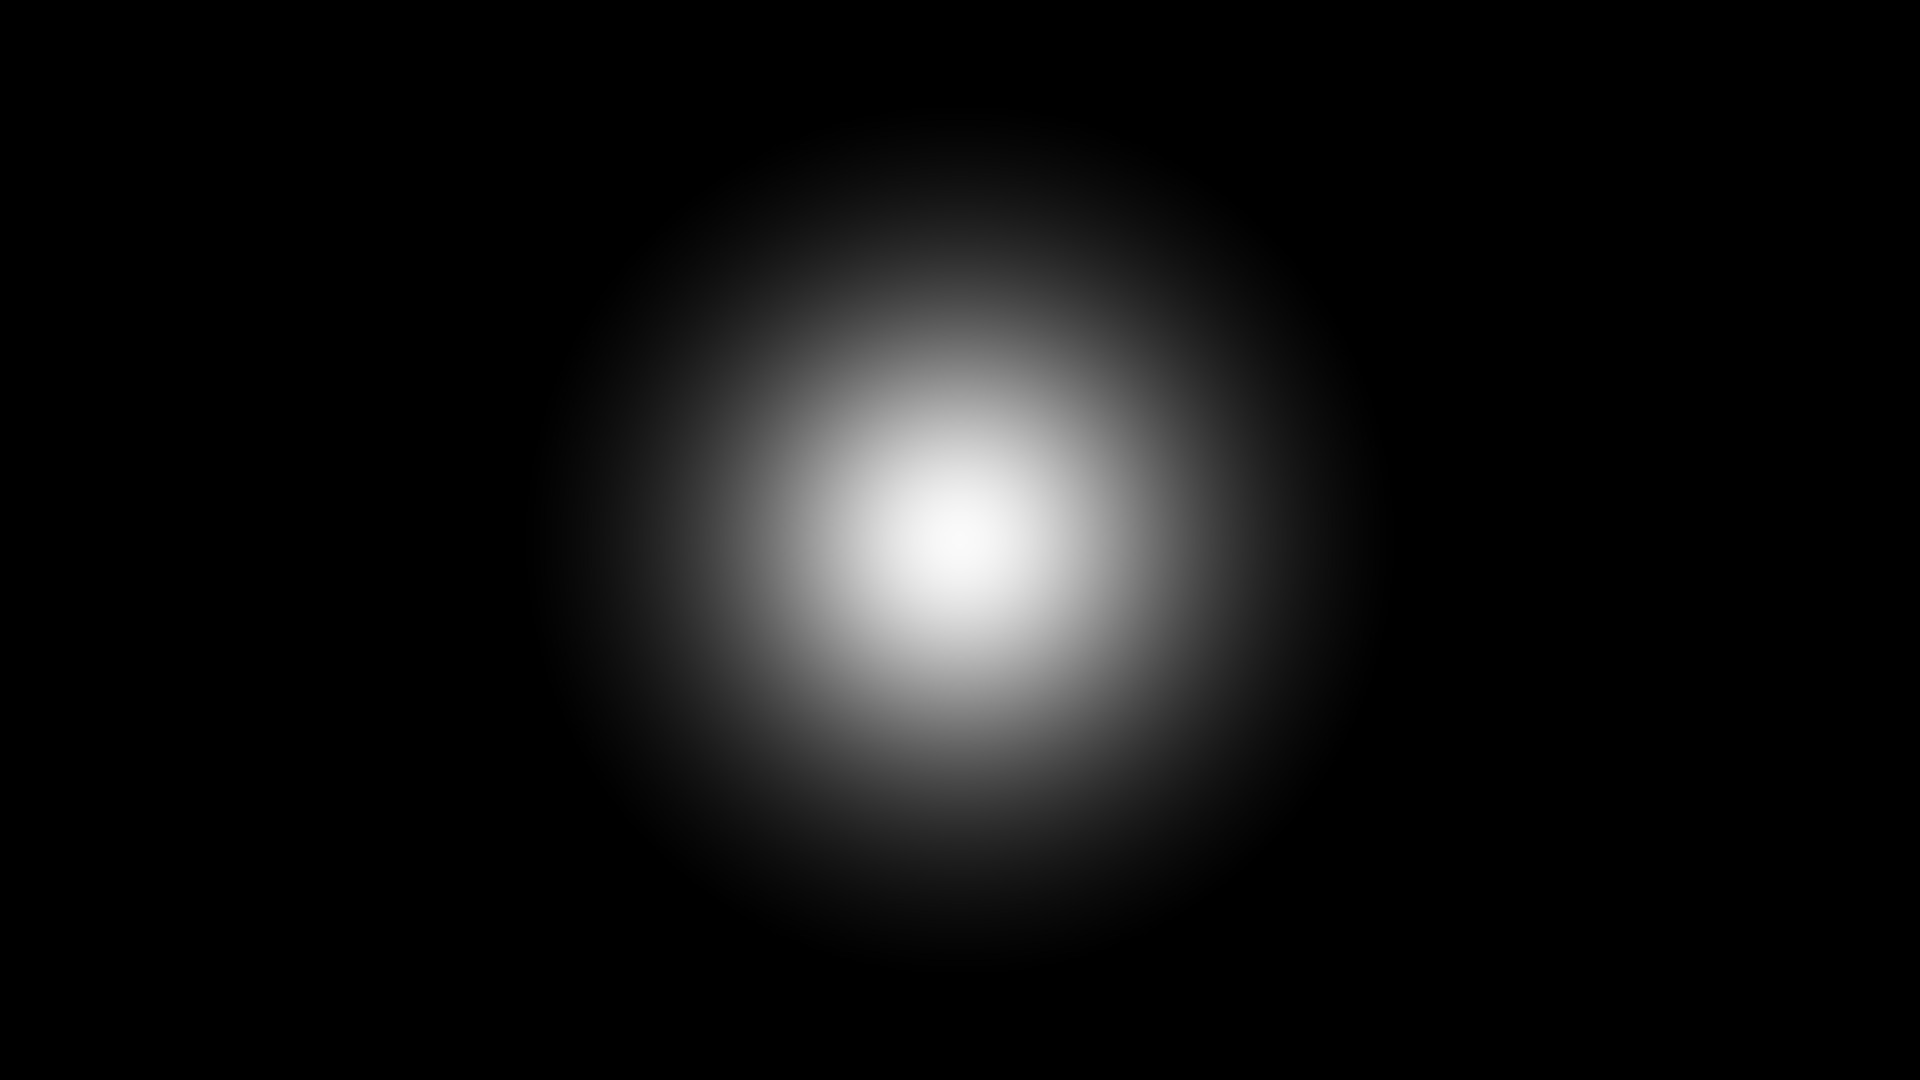
\includegraphics[width=0.3\textwidth]{chapters/ch3/img/light/output_07_1_0_0_1.png}}
\subfigure{
\includegraphics[width=0.3\textwidth]{chapters/ch3/img/light/output_07_1_0_02_1.png}}
\subfigure{
\includegraphics[width=0.3\textwidth]{chapters/ch3/img/light/output_07_1_0_05_1.png}}

\caption[Oświetlenie płaskiej powierzchni przez punktowe źródło światła]{Oświetlenie płaskiej powierzchni przez punktowe źródło światła. Obrazy w kolejnych kolumnach odpowiadają różnemu ustawieniu tego samego źródła względem płaszczyzny, zaś wiersze różnią się wartością $\cos\frac{\beta}{2}$ - idąc od góry 0,7; 0,85; 1,0 ($\cos\frac{\alpha}{2} = 0,7 = \mathrm{const}$). W przypadku, gdy $\cos\frac{\beta}{2}\neq\cos\frac{\alpha}{2}$, krawędź między obszarem oświetlonym a nieoświetlonym staje się rozmyta. Nieciągłości przejść między kolorami widoczne najbardziej w przypadku $\cos\frac{\beta}{2} = 0,85$ nie są wynikiem błędu algorytmu, a własności przetwarzania obrazu przez mózg człowieka - efekt ten zwany jest \textit{pasmami Macha}~\cite{MACH_BANDS}}
\label{ch3:img:light_comp}
\end{figure}